\documentclass[11pt]{article}

\usepackage[margin=1in]{geometry}
\usepackage[T1]{fontenc}
\usepackage[utf8]{inputenc}
\usepackage{lmodern}
\usepackage{microtype}
\usepackage{amsmath,amssymb,amsthm,mathtools}
\usepackage{booktabs}
\usepackage{array}
\usepackage{enumitem}
\usepackage{graphicx}
\usepackage{flafter}
\usepackage{float}
\usepackage{needspace}
\usepackage{xcolor}
\usepackage{natbib}
\usepackage[hidelinks]{hyperref}
\usepackage[nameinlink,noabbrev]{cleveref}
\hypersetup{
  pdftitle={Administered Menus and Focal Anchors: The Microstructure of the Market for Machine Intelligence},
  pdfauthor={Anonymous Authors}
}

\setlength{\emergencystretch}{3em}
\setlist{nosep,leftmargin=*}
\makeatletter
\renewcommand{\@seccntformat}[1]{\csname the#1\endcsname\hspace{0.6em}}
\makeatother

\newcommand{\E}{\mathbb{E}}
\newcommand{\Prb}{\mathbb{P}}
\newcommand{\1}{\mathbf{1}}
\newcommand{\OR}{\textsc{OpenRouter}}
\newcommand{\HF}{\textsc{Hugging Face}}
\newcommand{\pp}{\text{pp}}
\newcommand{\dd}{\mathrm{d}}

\title{Administered Menus and Focal Anchors:\\
The Microstructure of the Market for Machine Intelligence}
\author{Anonymous Authors}
\date{}

\begin{document}
\maketitle

\begin{abstract}
Open-weight models make it possible for many firms to sell inference under the
same model label.  Yet the resulting market is not a conventional spot market:
providers post sticky token-price menus, a router privately clears each request,
and displayed quotes can be refused when selected.  We construct a purpose-built
panel of provider-model quotes at five-minute frequency, router-published
operational aggregates, historical quote records, and randomized one-token
routing probes.  Two market facts and one power-gated operational design
characterize this market.  First, prices are
administered menus.  Only 2.8\% of provider-model-days reprice, changes are large,
93\% of quotes lie on cent grids, and state-dependent price gaps predict changes
out of sample while congestion does not.  Second, prices coordinate on a focal
anchor.  The two cheapest quotes tie on 45.9\% of multi-provider model-days,
versus 13.4\% in an independent grid-constrained null.  Where the model author
operates an endpoint, 65 of 72 tied minima equal the author's first-party price.
Third, a randomized-order crossover provides interim evidence that the router
manufactures firmness from revocable quotes.  In 76 complete four-policy blocks,
all-position default routing succeeds on 75 requests while three pinned
single-provider policies succeed on 61--64; 76 additional default-only monitoring
requests on different models are excluded.  These matched block rates are
secondary because earlier probes can affect later probes.  Carryover-robust
first-position outcomes remain masked until every arm reaches 500.  A steering
audit provides the mechanism link:
conditional on currently being cheapest, providers that cut price in the prior
week receive 3.9\% default selection share versus 23.3\% otherwise.  Thus the
observed rule does not reward past undercutting in the manner proposed to
discipline pricing algorithms.  The combined evidence supports a dealer-and-
dispatcher analogy rather than an automated-market-maker analogy: money prices
are sticky, quantity and eligibility clear at request time, and the platform's
substitution and prominence rules are first-order market-design instruments.
\end{abstract}

\section{Introduction}

The supply of machine intelligence has separated from model ownership.  A model
author releases weights or an API-compatible specification, independent inference
providers host the same model, and a routing platform presents those providers as
substitutable sources.  A user or application chooses the model label; the router
then chooses a provider, retries, or falls back.  This vertical separation creates
a market whose economic object is not simply ``which model is best?'' but ``how
does a platform clear multiple suppliers of the same model?''

That question is difficult to answer from posted prices alone.  The price surface
is public, but the allocation rule and capacity state are private.  The same cheap
quote can be visible to every user while being unavailable to a particular request.
Conversely, a router can deliver a high fill rate even if no individual quote is
firm, by substituting across providers.  Treating the public surface as an order
book therefore confuses displayed liquidity with delivered liquidity.  Treating
the router as a decentralized-exchange aggregator makes a related mistake: an
inference request is not atomically split across providers, the price is not an
executable commitment, and selection depends on hidden eligibility and quality.

We characterize the market with a measurement design that joins four kinds of
evidence: high-frequency quote surfaces, router-side operational aggregates,
historical price records, and our own randomized micro-purchases.  The design
keeps three estimands separate.  Public observations measure the displayed menu;
published operational aggregates measure congestion and enforcement; and owned
probes measure the realized policy for one account and workload.  None alone
identifies market-wide flow, private capacity, or provider cost.

The paper's contribution is two promoted empirical facts, a preregistered
firmness design with an interim block screen, and one mechanism audit.

\begin{enumerate}
  \item \textbf{Administered menus.} Prices move infrequently and by large
  increments.  A nested discrete-time hazard rejects a constant-hazard benchmark
  \citep{calvo1983}: duration and calendar effects matter, and the provider's
  price gap predicts repricing both in sample and on later days.  Rival changes
  improve the in-sample fit but not yet out-of-sample discrimination; congestion
  variables do not improve the hazard.  The money price is therefore a sticky
  menu, not the fast-clearing state variable.

  \item \textbf{Focal anchoring.} Minimum-price ties are too common to be a
  rounding artifact.  An independent grid-resampling null reproduces the observed
  price grid and heterogeneity but yields only a 13.4\% tie rate, compared with
  45.9\% in the data.  The focal level is economically interpretable: among tied
  models with an author-operated endpoint, 90.3\% tie at the author's first-party
  price.  This adapts the nonbinding-focal-point design of
  \citet{knittelstango2003} to a platform-defined reference price while stopping
  short of a collusion claim.

  \item \textbf{Power-gated manufactured firmness.} The money quote barely moves while
  operational state changes frequently.  A prospective crossover randomizes the
  order of default routing and three pinned-provider policies within model-time
  blocks.  In the 76 complete blocks, all-position default success is 98.7\%
  while pinned success is 80.3--84.2\%.  The common rejection level survives
  randomization of order, but an earlier apparent price-rank gradient does not.
  These are secondary matched-block rates: the primary first-position outcomes
  remain masked until 500 assignments per arm.  The design therefore suggests,
  but does not yet promote, router-manufactured firmness.

  \item \textbf{Steering memory.} \citet{johnsonrhodeswildenbeest2023} show
  that prominence rules which reward
  past price cuts can disrupt algorithmic collusion.  Our revealed-policy audit
  asks whether current cheapest providers receive more selection after a recent
  cut.  They receive less.  This is not proof of collusion--eligibility remains
  partly hidden--but it rejects the sign of the proposed pro-competitive
  implementation in the observed sample.
\end{enumerate}

These facts jointly imply a sharper market analogy.  The model is a product
standard or protocol; an inference provider is a dealer with a revocable quote
and hidden inventory; the router is a dispatcher and delegated purchasing agent;
and the harness is an application-side broker controlling retries and fallback.
The closest mature markets are request-for-quote dealer markets and platform
procurement, not constant-function automated market makers.  The analogy matters
because market quality depends on admission, substitution, and steering rules,
not only on quoted spreads.

Our results contribute to three literatures.  Work on language-model routing
optimizes quality-cost choice across models \cite{chen2023frugalgpt,
ong2024routellm,hu2024routerbench}; we instead measure competition and execution
among providers of the same model.  \citet{brownmackay2023} show how
heterogeneous pricing technology changes
competition; we provide the first high-frequency pricing-technology screen for
inference providers, while making its short-panel limits explicit.  Platform
design work studies prominence and algorithmic pricing
\citep{johnsonrhodeswildenbeest2023}; our audit turns its comparative static into a
statistic that a key-holder can reproduce from realized selections.

\section{Institutional setting and economic objects}
\label{sec:setting}

\subsection{The transaction}

A request names a model $m$, supplies an input, and may specify provider
preferences.  For provider $i$ at time $t$, the displayed menu contains an input
token price $p^{\mathrm{in}}_{imt}$ and an output token price
$p^{\mathrm{out}}_{imt}$.  For a fixed workload with $a$ input and $b$ output
tokens, the displayed money quote is
\begin{equation}
  q_{imt}(a,b)=a p^{\mathrm{in}}_{imt}+b p^{\mathrm{out}}_{imt}.
  \label{eq:quote}
\end{equation}
The platform can additionally observe health, throughput, latency, context-window
compatibility, account-specific limits, and contractual eligibility.  Let
$e_{imtu}\in\{0,1\}$ denote eligibility for user $u$, and let $c_{imt}$ denote
unobserved deliverable capacity.  The default router selects a provider according
to an unknown score
\begin{equation}
  i^*_{mtu}=\arg\max_i S(q_{imt},e_{imtu},c_{imt},z_{imt},h_u),
  \label{eq:score}
\end{equation}
where $z$ collects measured quality and $h_u$ is account state.  A pinned request
sets the candidate set to one provider and can disable fallback.  Comparing
default and pinned execution therefore measures the value of delegation, not
merely a price effect.

The request is served by one provider.  Fallback may create multiple attempts,
but this is sequential substitution rather than splitting one prompt across a
portfolio.  For the interfaces studied here, the route cannot generally be
observed as a firm executable allocation before purchase.  This absence of a
public pre-trade route is why literal order-flow front-running is not identified
from public data.

\subsection{Measurement levels}

We use an explicit observability hierarchy.  It prevents a common error in this
market: assigning the identifying content of realized flow to a price-only
simulation.

\begin{table}[H]
\centering
\small
\begin{tabular}{p{0.08\linewidth}p{0.25\linewidth}p{0.55\linewidth}}
\toprule
Level & Object & Identified use \\
\midrule
L0 & Public quote surface & Price levels, gaps, ties, grids, and repricing events \\
L1 & Documented policy simulation & Mechanical ranking or allocation proxy only \\
L2 & Public operational aggregates & Congestion, rate-limit, derank, and enforcement state \\
L3 & Owned realized requests & Selected provider, success, latency, cost, and fallback for the probed account \\
L4 & Provider or router logs & Capacity commitments, full attempt order, and cross-user flow \\
\bottomrule
\end{tabular}
\caption{Observability hierarchy.  The core paper uses L0--L3.  No claim that
requires cross-user order flow or private provider cost is made.}
\label{tab:levels}
\end{table}

Public token-allocation displays sometimes expose a deterministic price-weighting
proxy.  When a documented inverse-square proxy is available, we compute
\begin{equation}
  \widehat{s}_{imt}=\frac{q_{imt}^{-2}}{\sum_j q_{jmt}^{-2}}, \qquad
  \frac{\partial\log\widehat{s}_{imt}}{\partial\log q_{imt}}
  =-2(1-\widehat{s}_{imt}).
  \label{eq:simshare}
\end{equation}
Equation \eqref{eq:simshare} is a policy arithmetic identity.  It is not demand
elasticity and is never substituted for realized routing in our causal claims.

\section{Data and research design}
\label{sec:data}

\subsection{Capture system}

The live panel snapshots public provider-model menus every five minutes.  Each
record stores a UTC capture time, stable provider and model identifiers, input and
output token prices, capacity ceilings when displayed, and router-published
five- and thirty-minute enforcement aggregates.  Captures are append-only and
mirrored to remote object storage.  The analysis also uses a three-year historical
quote registry for lifecycle checks, public model-level token-allocation records,
and owned generation records for requests made with our study key.

The pricing freeze used in the main tables contains 2,968,449 endpoint snapshots
from 1,805 capture runs over nine days.  It covers approximately 300 models and 69
providers with enough exposure for provider-level cadence classification.  The
all-field event ledger contains 3,212 changes; the Brown--MacKay completion-price
screen retains 278 positive-price events spanning 7.53 days.  The public routing
simulation contains 562,550 provider-model-time rows over six days.  Owned legacy
traffic contains 2,659 raw rows over 65 runs; after deduplication and exclusion of
outcome-masked studies, 716 descriptive attempts remain and 617 identify the
selected provider.  The randomized crossover is a separate prospective release.

\begin{table}[H]
\centering
\small
\begin{tabular}{lrrp{0.36\linewidth}}
\toprule
Panel & Rows / attempts & Span & Primary role \\
\midrule
Endpoint snapshots & 2,968,449 & 9 days & Prices, grids, gaps, enforcement state \\
All-field price events & 3,212 & 9 days & Repricing incidence and event construction \\
Completion-price events & 278 & 7.53 days & Pricing-technology cadence screen \\
Public allocation proxy & 562,550 & 6 days & Mechanical share-price comparative statics \\
Legacy owned attempts & 716 & 65 runs & Descriptive provider-selection audit \\
Randomized crossover & 304 + 76 & prospective & 76 matched four-policy blocks plus default-only monitoring \\
Historical quote registry & multi-year & 3 years & Lifecycle and duration sensitivity \\
\bottomrule
\end{tabular}
\caption{Frozen analysis panels.  Sample sizes refer to the v3 manuscript
release and are updated only at registered promotion gates.}
\label{tab:samples}
\end{table}

\subsection{Cleaning and event construction}

Prices are converted to dollars per million tokens before comparisons.  We use
standard provider variants and remove exact duplicate captures.  A price event is
the first observation at which either token price differs from the preceding
observation for the same provider-model pair.  Five-minute timing creates interval
censoring within a capture bin; we do not infer within-bin order.  The first price
spell in a panel is left-censored and is excluded from moments that require age.

Operational counters are router-published aggregates, not raw request logs.
Their reporting can be intermittent.  Regressions that use utilization or
rate-limit state include a missingness indicator and are repeated on the
complete-reporting subsample.  Status-derived incidents are labeled as heuristics
unless the source publishes exact incident timestamps.  Owned probes record only
metadata needed for the study--assignment, policy, provider, latency, token count,
cost, and status--and never retain prompt payloads.

\subsection{Claim discipline}

The empirical sequence was adaptive, so we distinguish discovery from
confirmation.  Early descriptive analyses generated the administered-menu,
focal-anchor, and firmness hypotheses.  The fixed-order firmness pilot revealed a
large default-pinned gap but confounded policy with position.  We disclosed that
failure, froze a randomized-crossover replacement before observing its outcomes,
and treat the first release as interim.  Dynamic pricing results are re-estimated
at a registered 30-day gate using both the original and expanded vintages.  Tests
that have not reached their registered support are reported as power-gated rather
than as null findings.

\section{Fact 1: prices are administered menus}
\label{sec:menus}

\subsection{Frequency, size, and the clock}

Only 2.8\% of provider-model-days contain a price change.  Across completed
endpoint spells, the implied average duration is 26.7 days.  Conditional on a
change, the median absolute log change is 0.134; two thirds are cuts.  Ninety-three
percent of quotes lie on cent-per-million-token grids.  Twenty-six percent of cuts
occur at 00:00 UTC, a concentration difficult to reconcile with a continuously
clearing spot price and consistent with scheduled menu updates.

Raw pooled price-change kurtosis is 113 because providers and model scales differ.
After standardizing changes within provider, kurtosis is 3.54; the provider median
is 3.4 with interquartile range 2.1--4.9.  This statistic lies between a simple
state-dependent menu-cost benchmark and the Calvo benchmark discussed by
\citet{alvarezlebihanlippi2016}.  We use it as a sufficient-statistic diagnostic,
not as a structural estimate: the short panel leaves many providers with too few
changes for stable within-unit moments, and observation costs can mimic infrequent
adjustment \cite{alvarezlippipaciello2011}.

\subsection{A nested repricing hazard}

For provider-model pair $k$ on day $d$, let $Y_{kd}=1$ if a price changes.  We fit
a nested logit ladder
\begin{align}
 \Prb(Y_{kd}=1\mid X_{kd})
 &=\Lambda\big(\alpha + T_{kd}+G_{kd}+C_{kd}+R_{kd}\big), \label{eq:hazard}
\end{align}
where $T$ contains age and calendar terms; $G$ contains the absolute and signed
gap from the cheapest rival plus GPU-cost changes; $C$ contains published
utilization and rate-limit state; and $R$ contains rival raises and cuts in the
prior day.  The ladder adds these blocks sequentially.  Provider activity is
included as a frailty proxy, but with only nine days we do not estimate a full
unit-frailty duration model.

The constant-hazard model is decisively rejected by duration and calendar terms.
Adding price gaps improves fit ($p=1.0\times10^{-5}$); adding congestion does not
($p=0.17$); adding rival moves improves in-sample likelihood ($p=0.0018$).
Out-of-sample results are more disciplined.  On a day split, time dependence alone
has AUC 0.525 and the state-dependent model has AUC 0.638.  The strategic model has
AUC 0.555 on 36 test events.  Thus the gap channel survives temporal validation;
the rival-reaction channel does not yet generalize.

\begin{table}[H]
\centering
\small
\begin{tabular}{lccc}
\toprule
Hazard rung & Added state & Incremental evidence & Day-split AUC \\
\midrule
Constant & none & baseline & 0.500 \\
Time-dependent & duration, clock & rejects constant hazard & 0.525 \\
State-dependent & own-rival gap, GPU change & LR $p=1.0\times10^{-5}$ & 0.638 \\
Congestion & utilization, rate limits & LR $p=0.17$ & not promoted \\
Strategic & rival moves & LR $p=0.0018$ in sample & 0.555 \\
\bottomrule
\end{tabular}
\caption{Nested repricing hazard.  The strategic rung is labeled in-sample-only;
the 30-day both-vintage gate is preregistered.}
\label{tab:hazard}
\end{table}

The appropriate conclusion is narrower than ``providers use pricing
algorithms.''  Prices respond to their distance from the menu's competitive
reference point and are updated on scheduled attention dates.  We call them
administered menus because the money quote is set periodically while the physical
state clears elsewhere.  Whether rival reactions reflect common costs,
algorithmic competition, or coordinated behavior remains unresolved.

\section{Fact 2: minimum prices coordinate on an author anchor}
\label{sec:anchors}

\subsection{The tie atom and its null}

For each model-day with at least two providers, order the completion quotes and
define the relative second gap
\begin{equation}
  g_{md}=\frac{q_{(2),md}-q_{(1),md}}{q_{(1),md}}.
\end{equation}
Across 1,311 model-days, $g_{md}=0$ in 45.9\%.  A zero gap is especially common in
two-provider markets, but the atom persists in thicker markets.  Among all
non-minimum endpoint observations, 47.4\% are exactly tied at the minimum; the
remaining distribution has relatively little mass in very small undercuts.

Rounding can generate ties mechanically.  We therefore construct an independent
grid null.  Within each model-day, each provider draws a log-price deviation from
the pooled empirical distribution of deviations from model-day medians.  Draws are
independent across providers, added to the observed model-day median, and snapped
to the observed cent-per-million-token grid.  We preserve the observed number of
providers by model-day and repeat the procedure.  The null produces a 13.4\% mean
tie rate with 1.0 percentage-point simulation standard deviation.  Snapping to a
coarser dime grid increases the null to 27.6\%, still well below 45.9\%.  Because
the pooled deviation distribution retains some empirical tie mass, this null is
conservative with respect to independent coordination on the same grid point.

Post-freeze robustness (1,456 model-days, 148 model clusters) retains a 45.1\%
tie rate.  The cent-grid null is 12.9\%, giving a 32.2-point excess
(model-cluster bootstrap 95\% interval [25.8, 37.8]); the dime-grid null is
27.2\%, giving an 18.0-point excess [9.7, 25.1].  The bootstrap resamples whole
models and re-simulates the null within each draw; it is a robustness refresh,
not a replacement for the frozen v3 vintage.

\begin{table}[H]
\centering
\small
\begin{tabular}{lrr}
\toprule
Statistic & Estimate & Denominator \\
\midrule
Observed tie at minimum & 45.9\% & 1,311 model-days \\
Independent cent-grid null & 13.4\% & matched simulations \\
Independent dime-grid sensitivity & 27.6\% & matched simulations \\
Observed / cent-null ratio & 3.4 & -- \\
Observed / dime-null ratio & 1.7 & -- \\
\bottomrule
\end{tabular}
\caption{Minimum-price tie atom.  The null preserves market thickness, observed
deviation heterogeneity, and a discrete price grid, but breaks cross-provider
dependence.}
\label{tab:tienull}
\end{table}

\subsection{Identifying the focal level}

The latest snapshot contains 146 tied models.  For 72, the model author also
operates a first-party endpoint.  In 65 of those 72 cases, or 90.3\%, the tied
minimum equals the author's price to machine precision.  Sixty-one percent of tie
levels are round to a tenth of a dollar per million tokens, but roundness is not an
independent explanation: first-party author prices are themselves round.  Direct
provider APIs and router quotes are at exact parity in 99.6\% of matched cases;
we see almost no systematic direct-channel undercut.

The event directions complicate a collusion story.  Of 28 isolated tie formations,
71.4\% are formed by a downward move.  Of 38 isolated tie breaks, 86.8\% are broken
by a downward move.  Those directions are competitive.  The evidence therefore
supports an \emph{anchor}--a salient level on which independent providers cluster--
but does not identify why they anchor.  The author price may signal cost, quality,
or a voluntary most-favored-nation convention; it may also act as a Schelling-like
coordination device in the sense of \citet{knittelstango2003}.

The sharp discriminator is an author-price move.  If third-party ties re-form
around a new author price, the anchor is active; if they remain at the old level,
the tie is a launch fossil.  No author repricing occurs in the current nine-day
window, so the registered event study has zero treated events.  We report that
support failure rather than treating a stable anchor as evidence for either model.

\section{Interim design: does the router manufacture quote firmness?}
\label{sec:firmness}

\subsection{Price state and operational state}

Over the pricing panel, only 12\% of endpoints ever change price while 86\%
experience variation in published rate-limit state.  At thirty-minute horizons,
latency and enforcement variables load much more strongly on operational changes
than price does.  Raises tend to occur after slack rather than at congestion
spikes.  These facts suggest that scarcity is cleared through quantity,
eligibility, and fallback while the menu remains fixed.

Displayed unavailability is not enough to establish quote revocability: public
counters need not describe the study account.  We therefore purchase minimal
one-token completions under four policies.  Default routing delegates provider
choice and permits fallback.  Pinned-cheapest, pinned-second, and pinned-random
restrict the request to one provider selected from the contemporaneous public
surface.

\subsection{The failed pilot and randomized replacement}

The first 96 complete blocks always ran default first.  It found a 17.7 percentage-
point default advantage over the cheapest pinned quote, but order and policy were
perfectly confounded.  Account-level throttling, warm-up, or within-block
interference could produce the entire gradient.  We retain that result only as a
design failure.

The replacement randomizes both model order and policy order for every block and
records the assignment seed before execution.  Let $Z_{bp}$ be assignment of
policy $p$ to first position in block $b$, and $Y_{bp}$ request success.  Under
random assignment, the first-position difference
\begin{equation}
 \widehat{\tau}_{p}^{(1)}=
 \frac{\sum_b Z_{bD}Y_{bD}}{\sum_b Z_{bD}}
 -\frac{\sum_b Z_{bp}Y_{bp}}{\sum_b Z_{bp}}
 \label{eq:firstpos}
\end{equation}
is design-unbiased despite arbitrary effects of the first probe on later probes.
Pooled within-block contrasts are more precise but require that carryover is
controlled by randomized order and is not policy-specific after conditioning on
position.  We therefore report both and make the first-position estimator the
carryover-robust estimand at the promotion gate.

The frozen interim screen contains 76 complete four-policy blocks.  Every policy
therefore has 76 matched, randomized-order attempts: default succeeds on 75
(98.7\%), pinned-cheapest on 61 (80.3\%), pinned-second on 62 (81.6\%), and
pinned-random on 64 (84.2\%).  The collector also made 76 default-only monitoring
requests on four additional models.  Pooling those rows would produce 151/152,
but it would confound policy with model support; we exclude them.  Marginal Wilson
intervals in \cref{fig:core} are descriptive.  Random order balances clock
position, but treatment-specific carryover can still affect later positions.

The carryover-robust first-position analysis is outcome-masked until every arm
reaches 500 assignment-verified observations.  At the 2026-07-16 outcome-free
audit, the four counts are 15, 20, 19, and 22, with 100\% seed-replay success.
The eventual release uses the earliest chronological prefix satisfying the gate,
Holm-adjusted default-pinned randomization tests, and a prespecified rank-gradient
test.  Until then, the defensible interim conclusion is narrower: the approximately
19\% all-position pinned rejection level survives randomization of order and the
cheapest/second/random gradient is flat, but router-manufactured firmness is not
yet a promoted causal fact.

\begin{figure}[t]
\centering
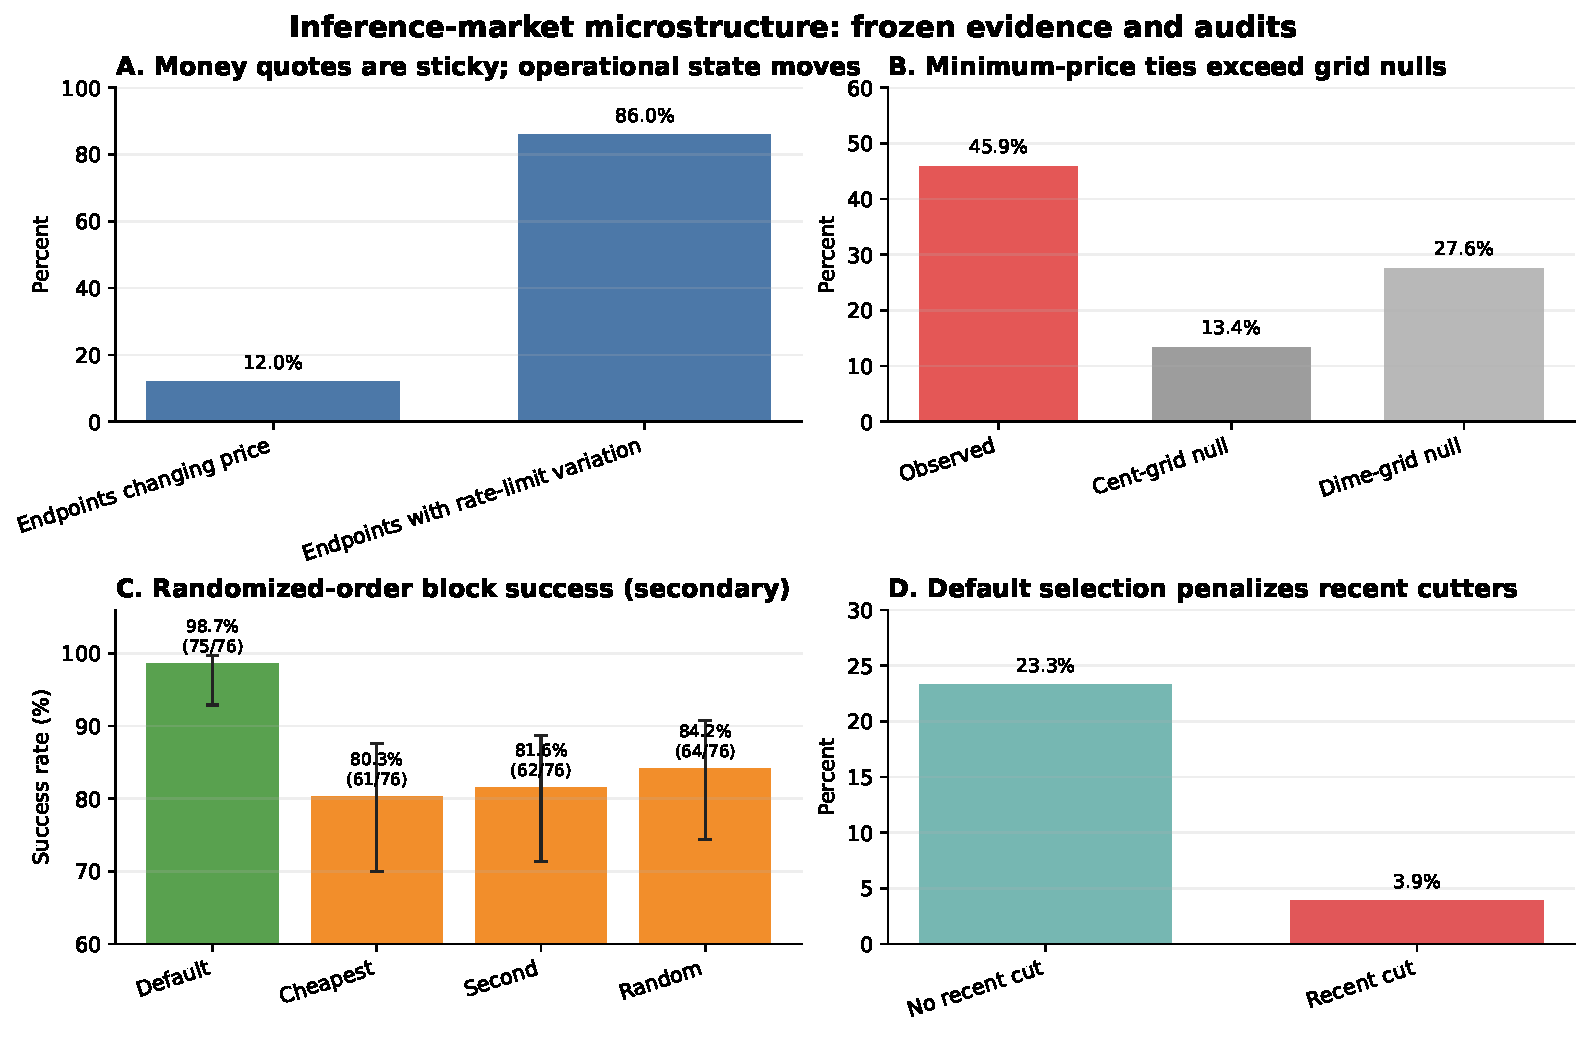
\includegraphics[width=\linewidth]{figures/core_facts.pdf}
\caption{Frozen evidence and audits.  Panel C shows secondary all-position rates
from 76 complete randomized-order blocks with marginal Wilson 95\% intervals;
the carryover-robust first-position outcomes remain masked until 500 assignments
per arm.  Panels A, B, and D are descriptive panel statistics.}
\label{fig:core}
\end{figure}

\section{The steering audit}
\label{sec:steering}

The platform-design problem is not exhausted by current-price ranking.
\citet{johnsonrhodeswildenbeest2023} study dynamic
price-directed prominence: a platform can reward a seller that previously cut
price with additional exposure, changing the repeated-pricing game even after the
current ranking is held fixed.  We turn the sign of that comparative static into a
revealed-policy audit.

For provider-model-day cell $(i,m,d)$, let $S_{imd}$ be its share of selected
providers among our default probes, $C_{imd}$ indicate a price cut in the prior
seven days, and $R_{imd}$ denote its current price rank.  The audit estimates
\begin{equation}
 S_{imd}=\alpha_{md}+\beta C_{imd}+f(R_{imd})+\varepsilon_{imd}
 \label{eq:steering}
\end{equation}
and reports the nonparametric cheapest-provider cells.  Among 251
provider-model-days, a currently cheapest provider without a recent cut has mean
selection share 23.3\%; one with a recent cut has 3.9\%.  The rank-controlled
coefficient is negative.  The observed policy therefore does not implement the
positive past-cut reward that disciplines patient pricing algorithms in the
theory.

Eligibility is the central threat.  Publicly quoted endpoints may be ineligible
for our region, prompt, or account.  Restricting the comparison to provider-model
pairs whose eligibility is independently confirmed by pinned probes preserves the
direction--30.0\% without a recent cut versus 9.5\% with a cut--but leaves only 11
and one cells.  We therefore label the unrestricted result an audit statistic, not
a causal effect of cutting price on future prominence.  Reversal would require
eligibility misclassification to be concentrated among recent cutters, a pattern
the prospective pinned panel is designed to measure.

Two interpretations remain.  Recent cuts may predict degraded capacity, causing
the router rationally to protect users.  Alternatively, a negative-memory rule
taxes price competition.  A randomized visibility test or router-side eligibility
log distinguishes them.  What the current data rule out is narrower but useful:
for this account and sample, the revealed selection pattern does not reward past
undercutting.

\section{Bounded secondary evidence}
\label{sec:secondary}

This section reports results that sharpen the market description but do not carry
the paper's novelty claim.

\subsection{Pricing cadence and Brown--MacKay}

Of 69 exposed providers, 19 reprice at least once: ten are classified intraday,
seven daily, and two weekly; 50 are inactive or left-censored.  Conditional on
model, slow providers quote 10.5\% more than fast providers.  The log-price
coefficient is $-0.0996$ with provider-clustered standard error 0.0292 and 95\%
interval $[-0.1569,-0.0424]$ across 5,576 observations and 131 models.

This resembles the cadence premium in \citet{brownmackay2023}, but the reaction
design is not supported.  Freezing cadence on the first 70\% of events leaves 21
evaluation waves and 124 rival risk pairs, with zero slow-initiator/fast-responder
exposures.  Adding reaction features slightly improves holdout MAE but not robust
discrimination.  The cadence premium is a resolved association; Brown--MacKay is a
power-gated competitive null, not the selected mechanism.

\subsection{Entry and long-memory demand}

Across 304 models, the elasticity of quoting-provider count with respect to token
demand is 0.149 (95\% interval $[0.126,0.175]$); the active-provider elasticity is
0.173.  Both are below i.i.d. square-root and cube-root entry benchmarks.  A
long-memory correction maps a measured multi-scale count Hurst exponent of 0.835
to $n^{(2-2H)/2}=n^{0.165}$, numerically close to the observed slope.  We treat this
as a remark, not identification: entry and demand are simultaneous, the panel is
short, and a deseasonalized intraday estimator is anti-persistent.  The registered
within-market interaction is underpowered.

\subsection{Retry feedback}

Within endpoint, subsequent thirty-minute request growth rises with the current
rate-limit share.  Demand-controlled OLS gives 0.167, while a backward placebo is
$-0.126$.  Instrumenting focal rationing with the same provider's rate limiting on
other models gives 0.023 with interval $[-0.043,0.085]$.  The sign-asymmetric OLS
is consistent with retry amplification; the instrument bounds the same-endpoint
component near zero and excludes the rerouting margin.  We do not convert either
coefficient into welfare because request aggregates do not reveal user values,
backoff policies, or cross-provider substitution.

\subsection{Conduct screens}

A naive event classifier labels 83\% of rival responses to cuts as
punish-and-revert.  Reconstructing the initiator's subsequent action changes the
classification: 42.1\% are punish-and-revert candidates and 41.1\% are cuts the
initiator later withdraws.  Among raises, 65.9\% are followed within 72 hours, but
many initiators have low measured volume.  These classifications show why posted-
price event shapes alone are not proof of algorithmic collusion.  Common cost
shocks, experimentation, and sparse observation remain observationally
equivalent without an adoption event or exogenous cost shock.

\section{Market-design implications and welfare}
\label{sec:welfare}

The facts identify design wedges, not a structural welfare number.  Let user type
$\theta$ have completion value $v_\theta$, delay cost $d_\theta$, and rejection
loss $\ell_\theta$.  If provider $i$ serves quantity $x_i$ with capacity $\mu_i$,
quality $a_i$, unit cost $c_i(a_i)$, and delay $W_i(x_i,\mu_i)$, a planner chooses
admission $A_\theta$, routing $x_{i\theta}$, capacity, and quality to maximize
\begin{align}
 \max \quad &\int A_\theta\left[v_\theta(1-r_\theta)
 -d_\theta W_\theta-\ell_\theta r_\theta\right]\dd F(\theta) \nonumber\\
 &-\sum_i\left[k_i(\mu_i)+c_i(a_i)x_i\right]
 -\int q_\theta(1-a_{i(\theta)})\dd F(\theta),
 \label{eq:planner}
\end{align}
subject to capacity, queue stability, and retry feedback.  Transfers cancel from
global welfare but determine participation and investment.

The decentralized agents solve different problems.  A provider chooses a sticky
menu, capacity, and hidden quality to maximize margin times routed volume minus
capacity and adjustment costs.  The router chooses admission, allocation,
fallback, monitoring, and steering to maximize fees and retained user value.  A
harness chooses model, retry, and fallback policies to maximize application
retention net of spend.  A user sees the harness's delivered price-quality-delay
bundle, not the provider market directly.

The evidence isolates four possible failures of decentralization.

\begin{enumerate}
  \item \textbf{Admission.} A high default fill rate can be privately valuable but
  socially excessive if retries impose congestion on other users.  User-value
  signals are needed to price or defer low-value requests.
  \item \textbf{Quality verification.} Selection on price and latency can induce
  unmeasured fidelity shaving.  The public panel has no task-level quality
  certificate, so the corresponding welfare term is unidentified.
  \item \textbf{Steering.} Prominence is an allocation instrument.  The negative
  past-cut association fails the sign of a known pro-competitive dynamic rule and
  may reduce the return to undercutting unless it is explained by hidden quality or
  capacity.
  \item \textbf{Retry feedback.} The OLS-placebo pattern is consistent with
  positive feedback, but the IV bound implies little same-endpoint amplification.
  The important unmeasured margin is rerouting across providers.
\end{enumerate}

The central market-design implication follows from observed quote revocability and
the platform's documented substitution role, not from a promoted causal effect.  A price-only
best-execution standard is incomplete when the quote is revocable.  A meaningful
score must combine expected money cost with success probability, latency, and
fidelity for a declared workload.  Capacity certificates, explicit fallback
prices, or auditable provider-level fill rates would move the market from displayed
menus toward executable commitments.  The companion mechanism paper studies such
certificates; this paper supplies the empirical reason they are needed.

\section{Related work}
\label{sec:related}

\paragraph{Model routing.}
FrugalGPT, RouteLLM, and RouterBench study how to choose among models with different
quality and cost \cite{chen2023frugalgpt,ong2024routellm,hu2024routerbench}.  Their
unit is a model.  Our unit is a provider-model endpoint, holding the model label
fixed and measuring the market that supplies it.  The two problems compose: a
harness may choose the model and a marketplace may then choose the supplier.

\paragraph{Pricing technology and focal points.}
\citet{calvo1983} provides the constant-hazard benchmark; observation and
menu-cost models motivate duration, gap, and change-size diagnostics
\citep{alvarezlippipaciello2011,alvarezlebihanlippi2016}.
\citet{brownmackay2023} show that heterogeneous repricing frequency can soften
competition.  \citet{knittelstango2003} identify a nonbinding
regulatory ceiling as a focal point.  We import their empirical logic but use an
author's first-party price as the candidate anchor and an independent discrete-grid
null as the counterfactual.

\paragraph{Platform steering and marketplace experiments.}
\citet{johnsonrhodeswildenbeest2023} connect
prominence rules to algorithmic pricing.  Our steering-memory statistic is an
empirical implementation of their sign restriction.  Switchback and marketplace
experiments require special care because treatment changes congestion and later
outcomes \cite{bojinov2023,holtz2025}; our first-position estimator protects the
firmness contrast from arbitrary within-block carryover.  Online matching under
stochastic rewards provides the OR analogue for provider selection
\cite{brubach2025}, but the inference setting adds sticky provider menus and hidden
eligibility.

\paragraph{Emerging AI-platform evidence.}
Recent work studies quality-adjusted AI prices and platform self-preferencing
\cite{wang2026,zhang2026}.  We complement these studies with provider-level
microstructure and a reproducible realized-policy audit.  The institutional APIs
are documented by the platforms themselves \cite{openroutermetadata,
hfinferenceproviders2026}; all policy claims in this paper are versioned to the
captured interfaces rather than generalized to undocumented behavior.

\section{Limitations and conclusion}
\label{sec:conclusion}

Five limitations define the claim boundary.  First, the main pricing panel is nine
days, so dynamic hazard and cadence results await the registered 30-day
both-vintage re-estimation; the outcome-free collection status is currently
10/30 dates.  Second, the randomized crossover's all-position block screen is
secondary, and its carryover-robust first-position counts are only 15--22 of 500
per arm.  Third, owned probes identify one
account, region, prompt family, and time window; they do not identify market-wide
provider shares.  Fourth, public operational fields are router-published
aggregates with missingness, not raw attempt logs.  Fifth, provider cost, private
rebates, task fidelity, and cross-user request order are unobserved.  We therefore
do not claim literal front-running, collusion, private cost, or a welfare loss.

Within those limits, the evidence changes the economic description of inference
markets.  Prices are not the rapidly clearing state variable.  Providers post
sticky administered menus and minimum quotes coordinate around the model author's
price.  The secondary block screen is consistent with the platform manufacturing
a firm service by substituting across revocable quotes, but that statement awaits
the first-position gate.  The platform's allocation memory does not reward recent
undercutting in the observed panel.  Even within these boundaries, the inference
router is a market designer: its admission, fallback, and steering rules determine
the delivered product as much as the visible price surface does.

The resulting research agenda is concrete.  Longer panels test whether gap-driven
repricing and author anchors survive new vintages.  The randomized promotion gate
estimates the deliverability frontier without order confounding.  Provider- or
router-side eligibility logs would separate rational quality protection from a
tax on undercutting.  Transparent decentralized markets supply an external
laboratory in which accepted bids and termination reasons are public.  Together,
these designs can turn a market that currently displays menus into one whose
commitments, allocation, and welfare can be audited.

\bibliographystyle{plainnat}
\bibliography{../references}

\appendix

\section{Variable construction and data-generating process}
\label{app:variables}

\begin{table}[H]
\centering
\footnotesize
\begin{tabular}{p{0.24\linewidth}p{0.68\linewidth}}
\toprule
Variable & Construction \\
\midrule
Completion quote & Output-token price in dollars per million tokens for the standard endpoint variant \\
Price event & First five-minute capture whose quote differs from the preceding same-endpoint capture \\
Cheapest rank & Dense rank of the workload-specific quote within model and capture time \\
Tie at minimum & At least two distinct providers have the exact minimum quote after common-unit conversion \\
Quote age & Time since the last observed event; first panel spell is left-censored \\
Recent cut & At least one negative completion-price event in the preceding seven calendar days \\
Default selection share & Selected-provider count divided by default probes in the provider-model-day cell \\
Rate-limit share & Router-published rate-limited count divided by successful plus rate-limited counts in the published window \\
Author-operated endpoint & Provider name matches the model author under the checked author-provider crosswalk \\
Direct parity & Direct API quote equals the contemporaneous router quote within machine tolerance \\
\bottomrule
\end{tabular}
\caption{Key variable definitions.}
\label{tab:variables}
\end{table}

The capture scheduler targets five-minute cadence, but network and source failures
create irregular intervals.  All duration variables use actual UTC timestamps.
Missing captures are never forward-filled for event timing.  A quote that is
unchanged across a gap contributes exposure but cannot locate an unobserved
intermediate round trip; historical sources are therefore used as a lifecycle
sensitivity, not to impute high-frequency paths.

The platform's five-minute and thirty-minute counters can overlap mechanically.
Regressions use one horizon at a time.  Capacity ceilings are displayed metadata,
not contractual commitments, and missing ceilings are not coded as infinite.
Derank transitions and rate-limit onsets are router enforcement events; they do not
reveal which user's request caused the event.

\section{Independent grid-null algorithm}
\label{app:gridnull}

For each observed model-day $(m,d)$ with $N_{md}\geq2$:
\begin{enumerate}
  \item Compute the observed median log price $\widetilde{p}_{md}$ and provider
  deviations $u_{imd}=\log p_{imd}-\widetilde{p}_{md}$.
  \item Pool deviations over model-days after the same endpoint and variant
  filters used by the observed statistic.
  \item Draw $N_{md}$ deviations independently with replacement, add
  $\widetilde{p}_{md}$, exponentiate, and snap to the declared grid.
  \item Record whether the two smallest simulated prices are equal.  Aggregate
  over model-days and repeat the full simulation.
\end{enumerate}
The primary grid is one cent per million tokens; the sensitivity is ten cents.
The simulation preserves the distribution of market thickness and model-day price
levels but removes cross-provider dependence.  Because the deviation pool is
empirical, it does not assume a parametric cost distribution.  Its main limitation
is that pooled deviations combine provider heterogeneity and may retain atoms from
the observed coordination process.

\section{Randomized-crossover protocol}
\label{app:crossover}

Each eligible block chooses a hot model with at least three publicly quoted
providers.  It freezes the contemporaneous provider set and computes cheapest,
second-cheapest, and random pinned candidates.  A deterministic pseudorandom seed
permutes the four policies and the model order.  The assignment row is written
before requests begin.  Requests use a fixed minimal prompt and one output token.

The primary outcomes are HTTP-level success and a valid generation identifier.
Secondary outcomes are latency, observed spend, selected provider, and fallback
attempts when exposed.  Missing cost is not recoded as zero.  A block is valid only
if assignment replay passes, the quote snapshot predates the request, and each
declared policy is attempted exactly once.  The confirmatory prefix stops at 500
valid attempts per pinned arm; later rows are a separate continuation sample.

The three primary hypotheses compare default success with each pinned arm.  The
family uses Holm adjustment.  Randomization inference permutes policy labels
according to the original assignment mechanism within blocks.  The first-position
estimator is primary for arbitrary carryover.  Pooled position-adjusted contrasts
and model-policy heterogeneity are secondary.  A flat cheapest/second/random
gradient is reported as evidence against rank-specific stale-quote refusal, not as
equivalence unless the registered equivalence margin is met.

\section{Steering-audit robustness}
\label{app:steering}

The unrestricted audit includes every provider-model-day that is currently
cheapest on the public surface and has at least one default probe.  Model-day fixed
effects remove common demand and quote-level shocks; price-rank controls compare
providers at the same current prominence.  Standard errors cluster at provider
and model-day in the promotion specification.

Three robustness layers are preregistered: (i) require at least one successful
pinned request for the provider-model pair; (ii) use only regions and prompt lengths
for which all compared providers pass eligibility; and (iii) instrument recent-cut
visibility with randomized quote-surface exposure if the platform permits a safe
visibility experiment.  Current data support the direction in layer (i) but not its
sample size.  No visibility instrument has fired.

\section{Transparent-compute comparator}
\label{app:akash}

A separately preregistered Akash study links public multi-provider bid sets, the
accepted lease, and exact on-chain termination reasons.  The launch backfill
replayed 2,929 retained closed leases with a 100\% exact-ID match.  Its
pre-preregistration support set contains 36 linked multi-provider choices: 20
accepted prices above the lowest bid and 16 at the lowest.  All 36 have the fixed
300-block follow-up, but only 20 close in that window; none records a provider,
escrow, or non-owner close.  This is zero-event support, not evidence of no effect.

The prospective cohort uses a second-snapshot inception rule, masks confirmatory
outcomes, and has a fixed release of 2026-08-15.  The comparator is excluded from
the paper's promoted facts because its market object is a compute lease rather than a
token-priced inference request.  Its role is methodological: it shows what becomes
identifiable when bids, acceptance, and termination are public.

\begin{figure}[H]
\centering
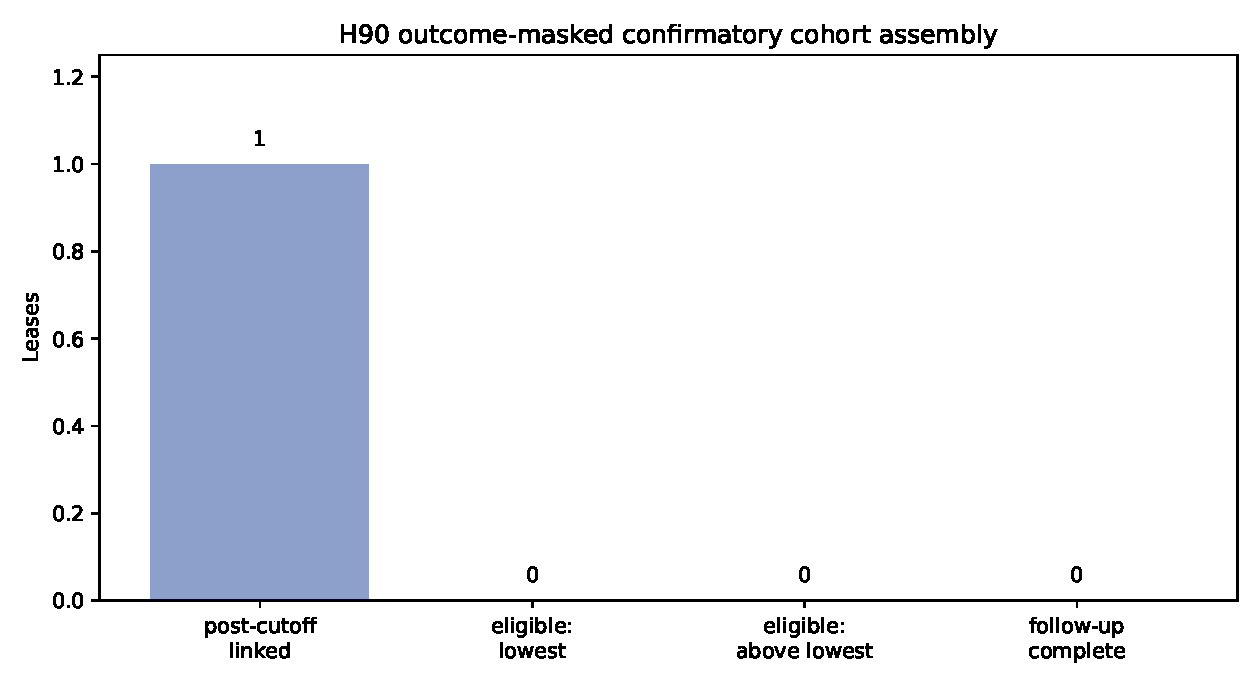
\includegraphics[width=0.62\linewidth]{../../analysis/h90_akash_contract_support.pdf}
\caption{Prospective Akash cohort assembly at launch.  The absence of eligible
post-cutoff observations is a support diagnostic; outcomes remain masked until the
fixed release.}
\label{fig:akashsupport}
\end{figure}

\section{Claim ledger and promotion gates}
\label{app:ledger}

\begin{table}[H]
\centering
\scriptsize
\begin{tabular}{p{0.22\linewidth}p{0.24\linewidth}p{0.22\linewidth}p{0.20\linewidth}}
\toprule
Claim & Current evidence & Missing identification & Promotion gate \\
\midrule
Administered menus & Frequency, size, grid, clock, day-split gap AUC & Long-run frailty and strategic response & 30 panel days, both vintages \\
Author focal anchor & Grid null and 65/72 author-price matches & Exogenous author move & First qualifying author repricing \\
Manufactured firmness & Secondary randomized-order block level, flat rank gradient & Carryover-robust first-position estimate and transport & 500 first-position assignments per arm \\
Negative steering memory & Rank-conditioned audit, same-sign eligibility subset & Complete eligibility or visibility instrument & Eligibility-complete panel \\
Brown--MacKay mechanism & Cadence premium & Slow-initiator/fast-responder exposure & 30 risk pairs after frozen cadence \\
Retry externality & Forward/backward asymmetry, small IV estimate & Cross-provider retry and user value & Incident instrument plus attempt logs \\
Literal front-running & None & Cross-user order and quote-update sequence & Negotiated router/provider event logs \\
Global welfare loss & None & Values, quality, costs, transfers, capacity response & Structural measurement contract \\
\bottomrule
\end{tabular}
\caption{The ledger distinguishes a supported market fact from the stronger
mechanism or welfare claim it may motivate.}
\label{tab:ledger}
\end{table}

\section{Reproducibility}
\label{app:repro}

All tables come from versioned Parquet and JSON artifacts carrying source and
retrieval timestamps and run identifiers.  Probe assignments record study and
block identifiers, seed, intended policy, position, and quote-snapshot key;
prompts and secrets are excluded.  The repository includes analyzers,
preregistrations, claim boundaries, and machine-readable summaries.  The
four-panel figure reads only frozen \texttt{paper\_estimates.json}, not the
pre-randomization legacy H80 summary.  The outcome-free
\texttt{manuscript\_promotion\_gate\_summary.json} freezes the nine-day and
earliest 30-day vintages and masks H80 outcomes until 500 first-position
assignments per arm.  Each gate release updates estimates, source manifest, and
PDF in one commit.

\end{document}
